\documentclass[presentation]{beamer}
%\documentclass[handout]{beamer}
\usetheme{Frankfurt}
\usecolortheme{seahorse}

\usepackage{amssymb}
\usepackage{amsmath}
\usepackage{graphicx}
\usepackage{subfigure}
\usepackage{multicol}
\usepackage[font={footnotesize,it}]{caption}

\usepackage{tikz}
\usetikzlibrary{graphdrawing,graphs} 
\usegdlibrary{layered}
\usegdlibrary{force}
\usegdlibrary{trees}

\usepackage{hyperref}

\begin{document}

\title{Using Time Series Models for Defect Prediction in Software Release Planning}
\author{James Tunnell \\
Central Washington University \\
Computational Science Program}
\date{June 5, 2015}

\begin{frame}
\titlepage
\end{frame}

\begin{frame}
\small{
\frametitle{Outline}
\tableofcontents[hideallsubsections] 
}
\end{frame}

\section{Introduction}

\begin{frame}
\begin{center}
\Large{Introduction}
\end{center}
\end{frame}

\subsection{Release Planning}

\begin{frame}[t]
\frametitle{Release Planning Objectives}
\begin{itemize}
\item{Two primary objectives of software release planning are:
  \begin{itemize}
    \item{Improving functionality}
    \item{Maintaining quality}
  \end{itemize}}
  \item{Both of these objectives are constrained by limits on development time and cost.}
\end{itemize}
\end{frame}

\subsection{Quality Control}

\begin{frame}[t]
\frametitle{Quality Control}
\begin{itemize}
  \item{Software defects (bugs) are inevitable}
  \item{Sufficient time should be available to ensure good quality (by testing and bug-fixing)}
  \item{Otherwise, there is a risk of
    \begin{itemize}
    \item{Low quality (failure to meet objective)}
    \item{Schedule slip (failure to respect constraint)}
    \end{itemize}
  }
  \item{This quality control (QC) time can be allowed for by limiting the scope of work in the planned release}
\end{itemize}
\end{frame}

\begin{frame}[t]
\frametitle{Quality Control (cont'd)}
\begin{itemize}
  \item{To support release planning, QC time can be estimated}
  \item{Assumption: QC time depends (at least partly) on the number of software defects introduced}
  \item{Then, a basis for estimating QC time would be the predicted number of defects}
\end{itemize}
\end{frame}

\subsection{Defect Prediction}

\begin{frame}[t]
\frametitle{Defect Prediction}
\begin{itemize}
  \item{Approaches to defect prediction tend to focus on either
    \begin{itemize}
    \item{Code analysis
      \begin{itemize}
      \item{Lines of code}
      \item{Number of decisions}
      \item{Code churn}
      \end{itemize}
    }
    \item{Historical information
      \begin{itemize}
      \item{Regression analysis}
      \item{Time series modeling}
	  \end{itemize}
	}
    \end{itemize}
  }
  \item{A multivariate time series model with exogenous inputs was chosen}
\end{itemize}
\end{frame}

%\subsection{Related Work: Using Code Analysis}
%
%\begin{frame}[t]
%\frametitle{Defect Prediction using Code Analysis}
%\begin{itemize}
%\item{Approaches using code analysis:
%  \begin{itemize}
%  \item{Akiyama used lines of code (LOC), number of decisions, and the number of subroutine calls \cite{1971_akiyama}}
%  \item{Gafney also used LOC \cite{1984_gaffney_estimating}}
%  \item{Henry and Kafura use information taken from design documents \cite{1984_henry_evaluation}}
%  \item{Nagappan and Ball use relative code churn (lines modified) \cite{2005_nagappan_codechurn}}
%  \end{itemize}
%}
%\item{These approaches all depend on specific design or implementation information}
%\item{This information is not available at the release planning stage}
%\end{itemize}
%\end{frame}
%
%\subsection{Related Work: Using Historical Information}
%
%\begin{frame}[t]
%\frametitle{Defect Prediction using Historical Information}
%\begin{itemize}
%\item{Approaches using historical information:
%  \begin{itemize}
%  \item{Li et al. extrapolate parameters of a regression model \cite{2004_li_emperical_eval}}
%  \item{Singh et al. use an ARIMA time series model \cite{2010_singh_predicting}}
%  \end{itemize}
%}
%\item{Both approaches are non-specific to design or implementation}
%\item{However, neither approach is explanatory}
%\end{itemize}
%\end{frame}

\section{Motivation}

\begin{frame}
\begin{center}
\Large{Motivation}
\end{center}
\end{frame}

\subsection{Release Plan Optimization}

\begin{frame}[t]
\frametitle{Release Plan Optimization}
\begin{itemize}
  \item{A release plan is formed by selecting features and improvements to work on}
  \item{Release plans can be compared by the expected revenue they will generate}
  \item{This optimization problem is posed as The Next Release Problem (NRP)}
\end{itemize}
\end{frame}

\begin{frame}[t]
\frametitle{Release Plan Optimization (cont'd)}
\begin{itemize}
  \item{The NRP is an abstract optimization problem}
  \item{In practice, QC time should be considered to ensure constraints are respected}
  \item{With the help of a defect prediction model, QC time can be estimated}
  \item{In this context, release plans are being compared}
  \item{For a defect prediction model to be useful, it should depend in some way on the basic elements of the release plan (planned new features and improvements)}
\end{itemize}
\end{frame}

\subsection{Explanatory Model}

\begin{frame}[t]
\frametitle{Explanatory Model}
\begin{itemize}
\item{Assumption: the number of defects in the future depends on more than just the number of defects in the past}
\item{A defect prediction model that depends only on previous numbers of defects is not explanatory}
\item{Such a non-explanatory model would always predict the same number of defects}
\end{itemize}

\begin{figure}[htbp]
\begin{center}
\tikz[nodes={text height=1em, text depth=.2em, draw=black!20, thick, fill=white, font=\small}, rounded corners, semithick]
  \graph[layered layout, level distance = 1cm, sibling sep = 1em]{
    "Release Plan 1" -> "Non-explanatory Model";
    "Release Plan 2" -> "Non-explanatory Model";
    "...." -> "Non-explanatory Model";
    "Release Plan N" -> "Non-explanatory Model";
    "Non-explanatory Model" -> "Predicted Defects";
  };
\caption{A non-explanatory model.}
\end{center}
\end{figure}
\end{frame}


\begin{frame}[t]
\frametitle{Explanatory Model (cont'd)}
\begin{itemize}
\item{A model could also depend on the key factors of a release plan}
\item{This would be an explanatory model structure}
\item{Such a model can potentially predict a different number of defects for every release plan}
\end{itemize}

\begin{figure}[htbp]
\begin{center}
\tikz[nodes={text height=1em, text depth=.2em, draw=black!20, thick, fill=white, font=\small}, rounded corners, semithick]
  \graph[layered layout, level distance = 1cm, sibling sep = 1em]{
    "Release Plan 1" -> "Explanatory Model";
    "Release Plan 2" -> "Explanatory Model";
    "...." -> "Explanatory Model";
    "Release Plan N" -> "Explanatory Model";
    "Explanatory Model" -> "Predicted Defects 1";
    "Explanatory Model" -> "Predicted Defects 2";
    "Explanatory Model" -> "...";
    "Explanatory Model" -> "Predicted Defects N";
  };
\caption{An explanatory model.}
\end{center}
\end{figure}
\end{frame}

\section{Time Series}

\begin{frame}
\begin{center}
\Large{Time Series Modeling}
\end{center}
\end{frame}



\subsection{Stationarity and Trends}

\begin{frame}[t]
\frametitle{Stationarity}
\begin{itemize}
\item{A stationary time series has time-invariant statistics}
\item{The time series models so far require time series to be stationary}
\item{Differencing a non-stationary series may produce a stationary series}
\item{Stationary can be determined by testing for trends}
\end{itemize}
\end{frame}

\begin{frame}[t]
\frametitle{Deterministic Trends}
\footnotesize{
\begin{itemize}
\item{A time series with a deterministic trend has a non-constant mean}
\item{The time series movements will generally follow the deterministic function}
\item{Fluctuations above or below this function are non-permanent}
\item{Such a time series is said to be stationary around a deterministic trend}
\end{itemize}
}
\begin{figure}[htbp]
\begin{center}
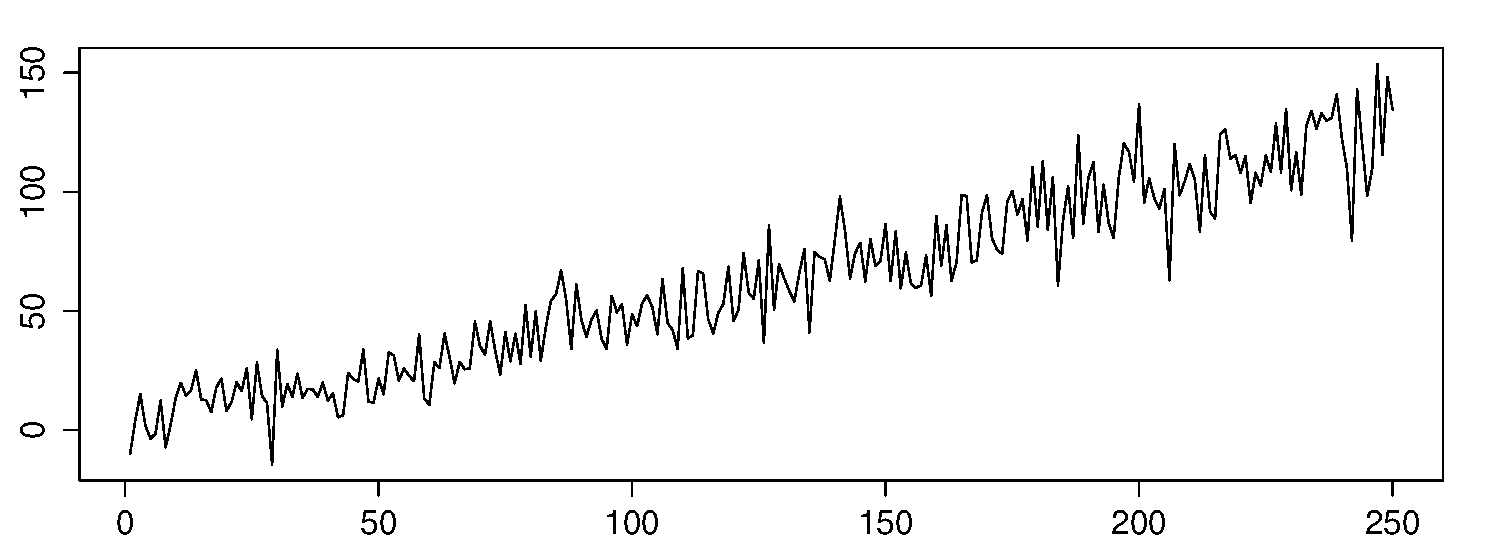
\includegraphics[width=\textwidth]{assets/deterministic_trend.eps}
\caption{Time series with a deterministic trend.}
\end{center}
\end{figure}
\end{frame}


\begin{frame}[t]
\frametitle{Stochastic Trends}
\footnotesize{
\begin{itemize}
\item{A stochastic trend shows permanent effects due to random variations}
\item{A series with stochastic trend will not necessarily fluctuate only close to the area of a deterministic function}
\item{A time series with stochastic trend is non-stationary}
\item{Differencing can be used to remove a stochastic trend}
\end{itemize}
}
\vspace{-.2cm}
\begin{figure}[htbp]
\begin{center}
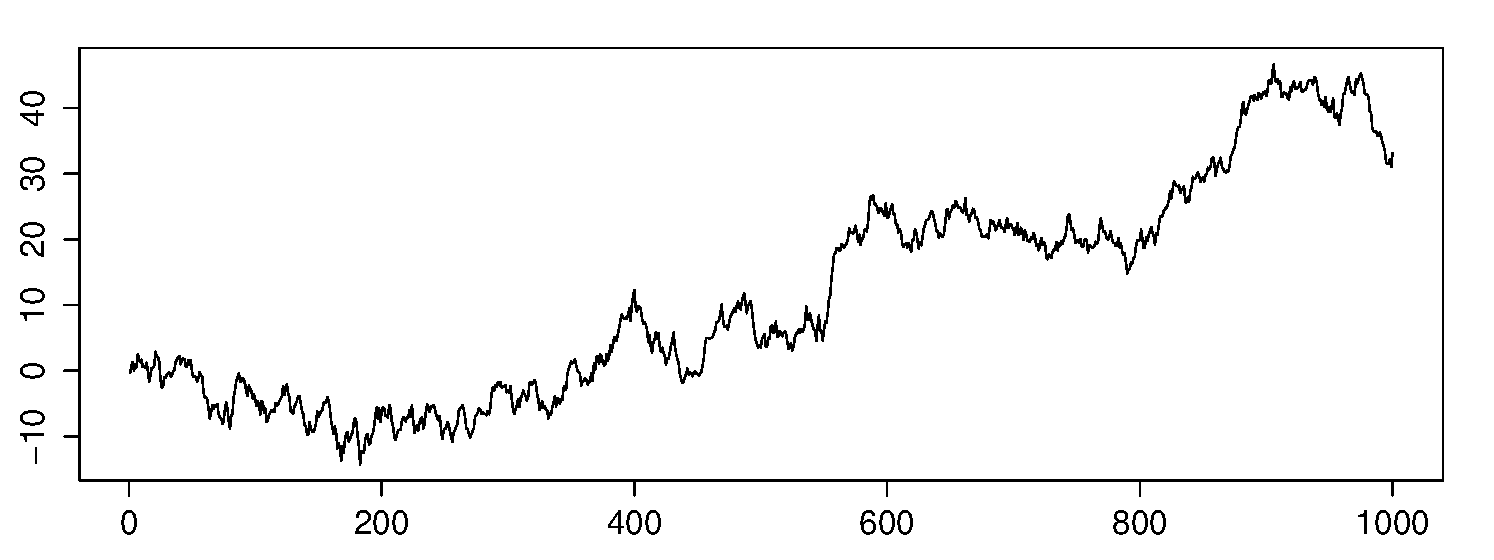
\includegraphics[width=\textwidth]{assets/stochastic_trend.eps}
\caption{Time series with a stochastic trend.}
\end{center}
\end{figure}
\end{frame}

\subsection{Stationarity Testing}

\begin{frame}[t]
\frametitle{Stationarity Testing}
\footnotesize{
\begin{itemize}
\item{A pure AR model of a time series with stochastic trend contains a unit root \cite{franses1998time}}
\item{Testing for the presence of a unit root can therefore be used to test for non-stationarity}
\item{A unit-root test starts with the null hypothesis that an AR model has a unit root}
\item{The alternative hypothesis is that an AR model of the time series does not have a unit root}
\item{Next, a test statistic is measured}
\item{If the p-value is below the chosen significance level, the null hypothesis is rejected}
\item{Rejecting the null hypothesis provides reason to accept the alternative hypothesis}
\item{The Augmented Dickey Fuller (ADF) test is commonly used for unit root testing}
\end{itemize}
}
\end{frame}

\begin{frame}[t]
\frametitle{Stationarity Testing (cont'd)}
\footnotesize{
\begin{itemize}
\item{On the other hand is a stationarity test}
\item{This test starts with the null hypothesis that a time series is stationary around a deterministic trend}
\item{If the test statistic is above some significance level, this shows that the null hypothesis can be accepted}
\item{Then the time series should be considered stationary}
\item{The Kwiatkowski-Phillips-Schmidt-Shin (KPSS) test can be applied for testing stationarity.}
\end{itemize}
}
\end{frame}

\section{Modeling Methods}

\begin{frame}
\begin{center}
\Large{Modeling Methods}
\end{center}
\end{frame}

\subsection{Overview}

\begin{frame}[t]
\frametitle{Time Series Modeling Methods}
\begin{itemize}
\item{Time series modeling methods typically involves
  \begin{enumerate}
  \item{Specification}
  \item{Estimation}
  \item{Diagnostic Checking}
  \item{Selection}
  \end{enumerate}}
\end{itemize}
\end{frame}

\subsection{Specification \& Estimation}

\begin{frame}[t]
\frametitle{Specification \& Estimation}
\begin{itemize}
\item{A $VARX(p)$ model is specified by choosing an order $p$}
\item{Model order is the number of autoregressive terms}
\item{This affects the number of parameters included in the model}
\item{To avoid having too many parameters relative to the number of observations, we use
  \begin{equation}
  p_{max} = \left \lfloor \frac{n}{m K_{min}} \right \rfloor
  \end{equation}
  
  \begin{itemize}
    \item{$n$ is the number of time samples}
    \item{$m$ is the number of time series}
    \item{$K_{min}$ is the minimum acceptable ratio of observations to parameters}
  \end{itemize}
  }
\item{Models parameters are estimated for orders $1, 2,..., p_{max}$}
\end{itemize}
\end{frame}


\subsection{Diagnostic Checking}

\begin{frame}[t]
\frametitle{Diagnostic Checking}
\begin{itemize}
\item{Diagnostics can tell if a model should be rejected}
\item{First diagnostic is for stability
  \begin{itemize}
  \item{AR model can have infinite impulse response}
  \item{To be stable, the roots of the characteristic equation must lie outside the unit circle \cite[p. 56]{box_jenkins_reinsel_2008}}
  \item{Equivalently, the inverse of the roots must lie inside the unit circle}
  \end{itemize}
}
\item{Next diagnostic is residual autocorrelation
  \begin{itemize}
    \item{Model residuals should be indistinguishable from white noise}
    \item{White noise is uncorrelated (no autocorrelation)}
    \item{Ljung-Box test forms a statistic from the autocorrelation of the residuals}
  \end{itemize}
}
\end{itemize}
\end{frame}

\subsection{Model Selection}

\begin{frame}[t]
\frametitle{Model Selection}
\begin{itemize}
\item{Model selection criteria are used to compare models according to their fit}
\item{Penalties for residual error and the number of parameters}
\item{Some common selection criteria
  \begin{itemize}
  \item{Akaike Information Criterion (AIC)}
  \item{AIC with correction (AICc)}
  \item{Bayesian Information Criterion (BIC)}
  \end{itemize}
}
\item{Parameter penalty is more severe for BIC and AICC than for AIC \cite{bisgaard2011time}}
\item{AIC will be used, since the number of parameters is already limited in the specification step}
\end{itemize}
\end{frame}

\section{Data Methods}

\begin{frame}
\begin{center}
\Large{Data Methods}
\end{center}
\end{frame}

\note{In this section, the data source and data collection method are detailed. Then, the method of preparing data for the modeling phase is presented.}

\subsection{Data Sources}

\begin{frame}[t]
\frametitle{Data source}
\begin{itemize}
\item{Data for time series modeling will be derived from project historical data}
\item{This historical data can be found in the project issue tracking system (ITS)}
\item{The issues in an ITS can be bugs, features, improvements, etc.}
\item{The basis for project selection is
\begin{itemize}
\item
Has been actively developed for at least several years
\item
Has openly available issue tracking system data
\item
Distinguishes between defects and other issue types
\end{itemize}}
\end{itemize}
\end{frame}

\begin{frame}[t]
\frametitle{Selected Projects}
MongoDB
\begin{itemize}
\item{A NoSQL, document-oriented database}
\item{The project has been actively developed since 2009}
\item{The \textit{core server} sub-project was chosen for modeling}
\item{Uses JIRA for issue tracking}
\item{Issue data was exported as XML}
\end{itemize}
\end{frame}

\begin{frame}[t]
\frametitle{Selected Projects (cont'd)}
Hibernate
\begin{itemize}
\item{An object-relational mapping (ORM) framework}
\item{The project has been actively developed since 2003}
\item{The \textit{orm} sub-project was chosen for modeling}
\item{Uses JIRA for issue tracking}
\item{Issue data was exported as XML}
\end{itemize}
\end{frame}

\begin{frame}[t]
\frametitle{Selected Projects (cont'd)}
NetBeans
\begin{itemize}
\item{A software development platform, including an IDE}
\item{The project has been actively developed as an open source project since 2000}
\item{The \textit{platform} and \textit{java} sub-projects were chosen for modeling}
\item{Uses Bugzilla for issue tracking}
\item{Issue data was extracted from MySQL database dump}
\end{itemize}
\end{frame}

\subsection{Data Cleansing}

\begin{frame}[t]
\frametitle{Data Cleansing}
\begin{itemize}
\item{Not all of the data was preserved for modeling}
\item{No-change issues
  \begin{itemize}
  \item{Only issues with resolutions such as \textit{fixed}, \textit{complete}, or \textit{done} were kept}
  \item{Other issues did not result in any change and were not included}  
  \end{itemize}
}
\item{Orphan sub-tasks
  \begin{itemize}
  \item{Issues that are sub-tasks are first converted to be the same type as the parent issue}
  \item{Sub-tasks whose parent issue is not in the dataset are considered orphans, and discarded}
  \item{Orphan sub-tasks can not be identified as improvement or new feature}
  \end{itemize}
}
\end{itemize}
\end{frame}

\subsection{Data Preparation}

\begin{frame}[t]
\frametitle{Data Sampling}
\begin{itemize}
\item{The dataset was operated on to prepare it for time series modeling}
\item{First, data was sampled at regular intervals, measuring
  \begin{itemize}
  \item{Number of bugs created}
  \item{Number of improvements resolved}
  \item{Number of new features resolved}
  \end{itemize}
}
\end{itemize}
\end{frame}

\begin{frame}[t]
\frametitle{Data Sampling (cont'd)}

\tiny{
  \begin{figure}[htbp]
  \begin{center}
  \begin{tikzpicture}[scale=.4]
    \tikzstyle{every node}=[font=\tiny]
    \node (bb) at (-2.5,2) [draw] {|Bug|};
    \node (n) at (-2.5,1) [draw] {|New Feature|};
    \node (ii) at (-2.5,0) [draw] {|Improvement|};
    \node (bbbb) at (-1,-1) [draw] {|Bug|};
    \node (i) at (0,-2) [draw] {|Improvement|};
    \node (bbbbb) at (1.4,-3) [draw] {|Bug|};
    \draw[dashed] (-3,3) -- (-3,-4);
    \draw[dashed] (0,3) -- (0,-4);
    \draw[dashed] (3,3) -- (3,-4);
    \draw (-4.5,3.5) node {Period 1};
    \draw (-1.5,3.5) node {Period 2};
    \draw (1.5,3.5) node {Period 3};
    \draw (4.5,3.5) node {...};
  \end{tikzpicture}
  \caption{Sampling example issue data.}
  \end{center}
  \end{figure}

  \vspace{.2cm}
  \begin{table}[htbp]
  \centering
  \begin{tabular}{ c | c | c | c }
  \hline
  Period & Improvements & New Features & Bugs \\
  ~& Resolved & Resolved & Created \\
  \hline
  1 & 0 & 0 & 1 \\
  2 & 1 & 1 & 1 \\
  3 & 1 & 0 & 1 \\
  \hline
  \end{tabular}
  \caption{Results of sampling example issues.}
  \end{table}
}
\end{frame}

\begin{frame}[t]
\frametitle{Establishing Stationarity}
\begin{itemize}
\item{Establish stationarity by testing
  \begin{itemize}
  \item{ADF unit root test}
  \item{KPSS stationariy test}
  \end{itemize}}
\item{If test results agree, then no differencing is necessary}
\item{Otherwise, difference data and retest}
\end{itemize}
\end{frame}

\begin{frame}[t]
\frametitle{Time Windowing}
\begin{itemize}
\item{Assumption: the software development process underlying a given project might change over time}
\item{The VARX model does not accommodate a changing process}
\item{To account for a changing process, data will be time windowed}
\item{Data will be used for modeling only if it occurs within the time window}
\item{This should limit the amount of process change the model is exposed to}
\end{itemize}
\end{frame}

\begin{frame}[t]
\frametitle{Time Windowing (cont'd)}
To still cover the entire dataset, the modeling methods are applied as the window advances by one sample . This is termed a \textit{sliding window}.
\begin{figure}[htbp]
\begin{center}
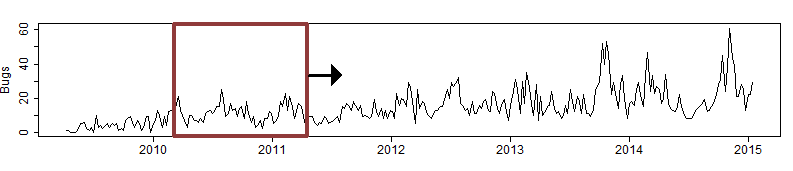
\includegraphics[width=\textwidth]{assets/time_series_sliding_window.png}
\caption{Sliding time window moves over the entire time series.}
\end{center}
\end{figure}
\end{frame}

\section{Results}

\begin{frame}
\begin{center}
\Large{Results}
\end{center}
\end{frame}

\subsection{Data Methods}

\begin{frame}[t]
\frametitle{Data collection results}
Summary of the collected data
\begin{table}
\centering
\scriptsize  
\begin{tabular}{c | c | c | c}
Project Product & Date Range & Initial Issue Count & Final Issue Count \\
Name &  & Count & Count \\
\hline
MongoDB \textit{core server} & Apr, 2009 - Jan, 2015 & 7,007 & 6,971 \\
Hibernate \textit{orm} & Apr, 2003 - Apr, 2015 & 14,262 & 8,278 \\
NetBeans \textit{platform} & Jan, 2001 - Jun, 2010 & 24,745 & 11,335 \\
NetBeans \textit{java} & Jan, 2001 - Jun, 2010 & 18,313 & 8,699 \\
\hline
\end{tabular}
\end{table}
It is worth noting that none of the datasets contained many orphaned subtasks.
The highest number found was 80 in the Hibernate \textit{orm} dataset.
\end{frame}

\begin{frame}[t]
\frametitle{Sampling Results}
Not knowing which sampling period would work best, sampling was performed for each of the
following sampling periods: 7 days, 14 days, and 30 days.

\begin{figure}[htbp]
\begin{center}
\includegraphics[width=.5\textwidth]{assets/hibernate_time_series_14.eps}
\caption{Time series data from sampling the Hibernate \textit{orm} dataset with a period of 14 days.}
\end{center}
\end{figure}

\end{frame}

\begin{frame}[t]
\frametitle{Stationarity Testing \& Differencing Results}
\begin{itemize}
\item
The time series were found almost without exception to be non-stationary.
\item
Differencing was found to remove nonstationarity
\item
Not knowing how differencing would affect model accuracy, data differencing of degrees of 0, 1, and 2 were made available for the modeling phase
\end{itemize}

\end{frame}

\begin{frame}[t]
\frametitle{Windowing Results}
Not knowing which window size would work best for the sliding window, a range
of window sizes were selected for each sampling period.

\begin{table}
\centering
\scriptsize  
\caption{Sliding windows sizes used}
\begin{tabular}{c | c}
Sampling Period & Sliding Window Sizes \\

\hline
7 days & 36, 39, 42, 45, 48, 51, 54, 57, 60, 63, 66, 69, 72, 75, 78 \\
14 days & 24, 27, 30, 33, 36, 39, 42, 45, 48, 51, 54 \\
30 days & 12, 15, 18, 21, 24, 27, 30, 33, 36 \\
\hline
\end{tabular}
\end{table}

\end{frame}

\subsection{Modeling Methods}

\begin{frame}[t]
\frametitle{Exploratory Results}
\begin{itemize}
\item{Modeling methods were first applied using the sliding window, in an exploratory fashion}
\item{Sampling period, window size, and degree of differencing are varied}
\item{Results are compared by the following metrics
\begin{itemize}
\item{The none-valid proportion}
\item{The non-normal proportion}
\item{Root-mean-square error (RMSE), which is the standard deviation of the error distribution}
\item{The in-interval proportion}
\end{itemize}
}
\item{First two metrics measure validity}
\item{Last two metrics measure accuracy}
\end{itemize}
\end{frame}

\begin{frame}[t]
\frametitle{Exploratory Results (cont'd)}
\begin{itemize}
\item
The only clear trend is that a higher degree of differencing results in lower model accuracy
\item
Other trends are not consistent for different sampling periods and across datasets.
\item
For a given dataset, the sampling period and window size can be chosen to maximize validity and accuracy.
\end{itemize}

\begin{figure}[htbp]
\begin{center}
\includegraphics[width=.5\textwidth]{assets/mongodb_pnonevalid_14}
\caption{An example of the inconsistent trends, from the MongoDB \textit{core server} dataset.}
\end{center}
\end{figure}

\end{frame}

\begin{frame}[t]
\frametitle{Exploratory Results (cont'd)}
Sliding window parameter values were selected based on results from exploratory modeling.

\begin{table}
\centering
\scriptsize  
\begin{tabular}{c | c | c | c}
Dataset & Degree of & Period & Window \\
~ & Differencing & ~ & ~ \\
\hline
MongoDB \textit{core server} & 1 & 14 & 24 \\
Hibernate \textit{orm} & 1 & 30 & 24 \\
NetBeans \textit{platform} & 1 & 14 & 27 \\
NetBeans \textit{java} & 1 & 14 & 30 \\
\hline
\end{tabular}
\end{table}

\end{frame}



\begin{frame}[t]
\frametitle{Final Results}
\begin{itemize}
\item{Final results were obtained by applying the sliding window approach to each dataset, using the parameter values from exploratory modeling.}
\item{The results are compared by
\begin{itemize}
\item{The none-valid and non-normal proportions}
\item{The distribution of actual compared to the distribution of predicted number of bugs}
\item{The distribution of prediction errors, with scale and shape being described by RMSE and Q-Q plot, respectively}
\item{The in-interval proportion for a 75\% or a 90\% prediction interval}
\end{itemize}
}
\end{itemize}
\end{frame}

\begin{frame}[t]
\frametitle{Final Results (cont'd)}
Summary of results
\begin{table}[htbp]
  \scriptsize
  \centering
  \begin{tabular}{ c | c | c | c | c | c | c }
  \hline
    & Window & None-valid & Non-normal &  & In 90\% & In 75\% \\
  Dataset & Count & Proportion & Proportion & RMSE & Interval & Interval \\
  \hline
  MongoDB & 126 & 2.38\% & 0\% & 14.7230 & 36.59\% & 27.64\% \\
  \textit{core server} &  &  &  &  &  &  \\
  Hibernate & 121 & 4.13\% & 0.86\% & 10.2685 & 53.91\% & 45.22\% \\
  \textit{orm} &  &  &  &  &  &  \\
  NetBeans & 219 & 9.59\% & 2.53\% & 15.2702 & 46.11\% & 39.38\% \\
  \textit{platform} &  &  &  &  &  &  \\
  NetBeans & 216 & 12.96\% & 14.89\% & 18.0469 & 43.13\% & 30.63\% \\
  \textit{java} &  &  &  &  &  &  \\
  \hline
  \end{tabular}
\end{table}
\end{frame}

\begin{frame}[t]
\frametitle{Final Results (cont'd)}
MongoDB \textit{core server} dataset
\vspace{-.65in}
\begin{figure}[htbp]
\begin{center}
\subfigure{
  \includegraphics[width=0.4\textwidth]{assets/mongodb/hist_forecast_errors}
}%
\subfigure{
  \includegraphics[width=0.4\textwidth]{assets/mongodb/qq_plot_forecast_errors}}\\ %
\vspace{-.2in}
\subfigure{
  \includegraphics[width=0.4\textwidth]{assets/mongodb/bugs_comparison}  
}%
\end{center}
\end{figure}
\end{frame}

\begin{frame}[t]
\frametitle{Final Results (cont'd)}
Hibernate \textit{orm} dataset
\vspace{-.65in}
\begin{figure}[htbp]
\begin{center}
\subfigure{
  \includegraphics[width=0.4\textwidth]{assets/hibernate/hist_forecast_errors}
}%
\subfigure{
  \includegraphics[width=0.4\textwidth]{assets/hibernate/qq_plot_forecast_errors}}\\ %
\vspace{-.2in}
\subfigure{
  \includegraphics[width=0.4\textwidth]{assets/hibernate/bugs_comparison}  
}%
\end{center}
\end{figure}
\end{frame}

\begin{frame}[t]
\frametitle{Final Results (cont'd)}
NetBeans \textit{platform} dataset
\vspace{-.65in}
\begin{figure}[htbp]
\begin{center}
\subfigure{
  \includegraphics[width=0.4\textwidth]{assets/netbeans/platform/hist_forecast_errors}
}%
\subfigure{
  \includegraphics[width=0.4\textwidth]{assets/netbeans/platform/qq_plot_forecast_errors}}\\ %
\vspace{-.2in}
\subfigure{
  \includegraphics[width=0.4\textwidth]{assets/netbeans/platform/bugs_comparison}  
}%
\end{center}
\end{figure}
\end{frame}

\begin{frame}[t]
\frametitle{Final Results (cont'd)}
NetBeans \textit{java} dataset
\vspace{-.65in}
\begin{figure}[htbp]
\begin{center}
\subfigure{
  \includegraphics[width=0.4\textwidth]{assets/netbeans/java/hist_forecast_errors}
}%
\subfigure{
  \includegraphics[width=0.4\textwidth]{assets/netbeans/java/qq_plot_forecast_errors}}\\ %
\vspace{-.2in}
\subfigure{
  \includegraphics[width=0.4\textwidth]{assets/netbeans/java/bugs_comparison}  
}%
\end{center}
\end{figure}
\end{frame}



\section{Conclusion}

\begin{frame}
\begin{center}
\Large{Conclusion}
\end{center}
\end{frame}

\subsection{Discussion}

\begin{frame}[t]{Discussion}
\begin{itemize}
\item{Windowing was used to maximize validity and accuracy}
\item{Validity
\begin{itemize}
\item{None-valid proportions were between 2\% and 13\%}
\item{Non-normal proportions were between 0\% and 15\%}
\item{Together, these proportions represent the risk that for any given sample
window there will be no valid course for making a prediction}
\end{itemize}}
\item{Accuracy
\begin{itemize}
\item{in-interval proportions at a 90\% prediction interval were between 36\% and 54\%}
\item{in-interval proportions at a 75\% prediction interval were between 27\% and 46\%}
\item{RMSE was between 2.40 and 9.02 bugs per week}
\item{The best results were for the Hibernate \textit{orm} dataset}
\end{itemize}
}
\end{itemize}
\end{frame}


\begin{frame}[t]{Discussion (cont'd)}
\begin{itemize}
\item{The sliding window provides control over validity and accuracy}
\item{It also conveys a picture of how a model can generally be expected
to perform for any given window in the future}
\end{itemize}

\begin{table}[htbp]
\centering
\scriptsize
\begin{tabular}{ p{.35\textwidth} | p{.6\textwidth} }
  \hline
  Modeling Results & Future Expectation \\
  \hline
  Low invalidity proportions & A valid model will likely be available \\
  High in-interval proportion & Model prediction will likely not exceed prediction interval \\
  Low RMSE & Model prediction error will likely be low \\
  \hline
\end{tabular}
\end{table}

\end{frame}


\begin{frame}[t]{Future Work}
Possible future research:
\begin{itemize}

\item{Use change management data in a time series model
\begin{itemize}
\item{Problems with issue tracking system (ITS) data:
\begin{itemize}
\item{Subject to human error (unknown lag time before changes are entered)}
\item{Information is lost (change magnitude, location(s), author)}
\end{itemize}}
\item{ITS data for changes made (new features, improvements) can be replaced with change management data}
\end{itemize}
}

\item{Use birth-death process models
\begin{itemize}
\item{The issue tracking system data will always be non-negative, since it is count data}
\item{A birth-death process specifically models count data, being used for population size}
\item{Does not require sampling or differencing}
\item{Could directly model issue creation (birth) and resolution (death)}
\end{itemize}
}

\end{itemize}
\end{frame}


\begin{frame}[t]{Thanks \& Questions}
\begin{itemize}
\item{CS Faculty
\begin{itemize}
\item{Dr. Razvan Andonie}
\item{Dr. Filip Jagodzinski}
\item{Dr. John Anvik}
\end{itemize}
}
\item{Math Faculty
\begin{itemize}
\item{Dr. Yvonne Chueh}
\item{Dr. Kathryn Temple}
\end{itemize}
}
\end{itemize}
\end{frame}

\section{References}

\begin{frame}[allowframebreaks]{References}
\begin{center}
\bibliography{../references}
\bibliographystyle{abbrv}
\end{center}
\end{frame}

\end{document}
